% !TEX root = ../CINTA-cn.tex
%%%%%%%%%%%%%%%%%%%%%%%%%%%%%%%%%%%%%%%%%%%%%%%%%%%%%%%%%%
% Author: Libin Wang
% This document was released as open source on 2026-06-18.
% Chapter 5. Miller-Rabin Primality test
% Copyright 2023, Libin Wang. Creative Commons License
% This work is licensed under a Creative Commons Attribution-NonCommercial-NoDerivatives 4.0 International License.
%%%%%%%%%%%%%%%%%%%%%%%%%%%%%%%%%%%%%%%%%%%%%%%%%%%%%%%%%%

\chapter{素数与素性测试}
\label{chap:prime} 
\begin{introduction}
  \item 素数的若干定理
  \item Carmichael 数
  \item 米勒测试
  \item 米勒-拉宾算法
\end{introduction}

素数在数学中类似空气存在于地球，无处不在而且非常重要。本章首先简要地陈述素数的若干性质，为以后章节铺垫基础，然后重点讲解一种判断整数是否素数的算法。
\section{素数}
\label{sec:prime}
以下列举若干关于素数的定理与结论，都是一些常识。

\begin{theorem}{算术基本定理}{fta} \index{fundamental theorem of arithmetic} \index{算术基本定理}
%\label{thm:fta}
每一个自然数都可唯一地表达为素数的乘积。
\end{theorem}

\begin{theorem}{欧几里得定理}{euclid2}
%	\label{thm:euclid2}
素数有无穷多。
\end{theorem}
\begin{proof}
	使用反证法。假设只存在有限多的素数，比如$p_1$，$p_2$，$\ldots$，$p_n$，记$N = p_1 p_2 \cdots p_n + 1$。
	根据条件假设，$N$必为合数，所以存在某个$p_i$，$ 1 \leq i \leq n$，使得$p_i \mid N$。则$p_i$必定整除$N - p_1 p_2 \cdots p_n = 1$，但是
	这是不可能的。因此，或者$N$是素数，或者存在另一个素数$q \neq p_i$，$ 1 \leq i \leq n$，$q\mid N$。
\end{proof}
	
简单的计算可知，素数分为两类，一类模$4$余$1$，一类模$4$余$3$。
\begin{theorem}{模$4$余$3$的素数}{mod_4_3}
模$4$余$3$的素数有无穷多。
\end{theorem}

\begin{proof}
反证法。假设模$4$余$3$的素数有限多，可枚举出所有模$4$余$3$的素数构成以下集合：
\[S = \{3, p_1, p_2, \ldots, p_n\}\]
令
\begin{equation}
\label{eq:mod4_3}
P = 4p_1p_2 \cdots p_n + 3
\end{equation}
则$P$可被分解为一系列素数的乘积，
\begin{equation}
\label{eq:mod4_3_1}
P = q_1 q_2 \cdots q_m
\end{equation}
如果所有的$q_i$都模$4$余$1$，则$P$必然模$4$余$1$，然而从$P$的构造可知，$P$模$4$余$3$，
所以，必然存在某个$q_i$模$4$余$3$。最后要证明$q_i \notin S$。由等式~\ref{eq:mod4_3}可知，$S$中的元素都不整除$P$，
但是等式~\ref{eq:mod4_3_1}说明，$q_i$整除$P$。所以，$q_i \notin S$，即找到了一个新的模$4$余$3$的素数，
假设不成立！\qed
\end{proof}

\begin{thinking}
利用以上证明方法能证明模$4$余$1$的素数有无穷多吗？请大家尝试，并发现证明的难点。
\end{thinking}

%Todo 素数基本定理
欧几里得定理告诉我们，素数有无穷多，需要进一步问，素数到底有多少，其分布如何？
通过简单的 Sage 命令，我们可以稍微建立起一些关于素数分布的基本认识。
\begin{lstlisting}
sage: prime_pi(1000)
168
sage: prime_pi(10000)
1229
sage: prime_pi(65537)
6543
sage: plot(prime_pi, 1,10000, rgbcolor=(0,0,1))
\end{lstlisting}

以下是用 Sage 命令画出的一万以内整数中的素数分布图，大家可以尝试使用其他参数，取$1000$或者$100,000$等
得到的效果图基本相同。
%Add 20200723
\begin{figure}
\begin{center}
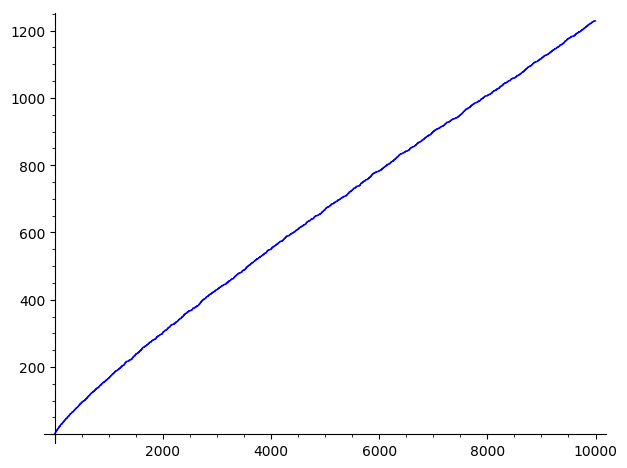
\includegraphics[scale=.5]{figures/prime.jpg} 	
\caption{一万以内整数的素数分布图}
\label{fig:prime}       % Give a unique label
\end{center}
\end{figure}

%20211230, from Raji IENT
然而素数的分布特性往往超出了我们的想象。以下定理说明，存在任意大的整数区间里面一个素数都没有。
即说明素数的空间呈现出一种不规则特性。
\begin{theorem}{素数的分布}{composite}
%	\label{thm:composite}
对任意的正整数$n$，存在$n$个连续的合数。
\end{theorem}
\begin{proof}
对任意的正整数$n$，
构造如下$n$个连续的整数序列：
\[(n+1)! + 2, (n+1)! + 3, \ldots, (n+1)! + (n+1) \]
因为，容易看出，对任意的正整数$k$，如果$2 \leq k \leq n+1$，则$k$整除$(n+1)! + k$。\qed
\end{proof}

以下两个定理都属于常识，但是，并非所有的常识都容易证明。
要证明它们需要使用解析数论、复分析等知识，已超出本书的教学范围。
%Todo: To give  intuition
\begin{theorem}{狄利克雷定理.}{Dirichlet}
设$a, m \in \Z$，且$\gcd(a,m)=1$，则存在无穷多个模$m$同余$a$的素数。即有无穷多素数满足：
\[ p \equiv a \pmod{m}.\]
\end{theorem}
定理~\ref{thm:mod_4_3}显然是狄利克雷定理的一个特例。该定理由大名鼎鼎的高斯提出，而首先由狄利克雷证明。

\begin{theorem}{素数定理}{prime}
%	\label{thm:prime}
函数$\pi(x)$渐进于$x/\log(x)$，即：
\[ \lim_{x \to  \infty}\frac{\pi(x)}{x/\log(x)} = 1\]
\end{theorem}
素数定理刻画素数的分布，对一个足够大的正整数$x$，给出所有小于$x$的素数的个数的一种近似值，而你并不需要去找出所有这样的素数。

以下常识则属于暂时
尚无法证明也无法证伪的猜想。
\begin{conjecture}{歌德巴赫猜想}{goldbach}
任意的偶数$n \geq 4$都是两个素数之和。
\end{conjecture}

\begin{conjecture}{孪生素数猜想}{twin_prime}
有无穷多的素数$p$使得$p+2$也是素数。
\end{conjecture}

\begin{conjecture}{$N^2+1$猜想}{n2_1}
有无穷多的素数形如$N^2+1$，$N \in \N$。
\end{conjecture}

\section{素性测试}
\label{sec:primeTest}
本节讨论素性测试问题，即如何判断一个大的奇整数$n$是否素数。先看以下 Sage 实例。
\begin{example}
\label{exm:prime}
\begin{lstlisting}
sage: is_prime(131)
True
sage: is_prime(12345678987654321)
False
sage: is_prime(969012308683094185386857784379)
True
sage: time is_prime(969012308683094185386857784379)  #考察算法的执行时间
CPU times: user 6.18 ms, sys: 1.31 ms, total: 7.5 ms
Wall time: 7.57 ms
True
\end{lstlisting}
\end{example}

这个问题似乎并不难，因为大家都熟悉这样一种简单的方法--\emph{试除法}（\emph{trial division}），代码如下：
\begin{center}
	\lstinputlisting[caption = 试除法]{codes/NaiveIsPrime.c}
\end{center}

为什么我们对试除法并不满意？对特定的输入值$n$，试除法的复杂性是$\mathcal{O}(\sqrt{n})$，显然一个多项式时间算法。
按常识而言，这是高效算法。然而，在这里需要用另一种方式看待算法的复杂性。

某些特定的算法，往往并不关心
某个特定的输入值，而关注满足某一个规模的输入值，此时衡量算法的复杂性的输入就应该是输入值的数据长度。
以素性测试问题为例，算法并不关心某个输入值$n$是否素数，而是关注某一类整数，比如$\lambda$比特的所有整数。
此时衡量算法复杂性的参数应该是$\lambda$而不是$n$。因为试除法的复杂性是$\mathcal{O}(\sqrt{n})$，以
$\lambda$为考量指标代入，则变成了$\mathcal{O}(\sqrt{2^{\lambda}})$，这是以$\lambda$为参量的指数式复杂性。

考虑具体的数值，如果要判断某个
$100$比特的整数是否素数，用试除法的话，最多要做$2^{50}$次除法，使用一般的计算机很难算出答案。
即使是超级计算机也不可能具有例子~\ref{exm:prime}中展示出来的秒杀速度。
在算法理论中，把试除法这种
貌似多项式时间的复杂性称为\emph{伪多项式时间}（\emph{pseudo-polynomial time}）
\index{伪多项式时间}\index{pseudo-polynomial time}。所以，需要设计更高效的素性判定算法。

以下介绍一种最常用的高效的素性判定算法，其思想很简单，源自于费尔马小定理。
费尔马小定理告诉我们，如果$p$是素数，对任意$a \in \Z$且$p \nmid a$，以下等式成立：
\begin{equation}
\label{eq:fermat_eq}
a^{p-1} \equiv 1 \pmod{p}
\end{equation}
如果上式不成立，则$p$必然是合数。
反过来，如果上式成立，不能论断$p$一定是素数，只能说没有发现\emph{证据}证明$p$是合数，
也就是，$p$可能是素数。假设能以比较大的概率找到$p$是合数的证据，
只需要选不同的$a$，不断判断等式~\ref{eq:fermat_eq}是否成立，
如果多次判断而又找不到$p$是合数的证据，则说明$p$以很大的概率是一个素数。请大家相信概率！
这样，通过判断等式~\ref{eq:fermat_eq}是否成立为判断一个整数是否素数提供了思路。

\begin{example}
设$p=51$，计算可知：
\[2^{50} \equiv 4 \pmod{51}\]
所以，$2$是$51$不是素数的一个证据。
但是，
\[16^{50} \equiv 1 \pmod{51}\]
$16$则提供一个让$51$看上去像是一个素数的“伪证据”。同时提供“伪证”的还有$35$。
\end{example}

存在伪证已经颇糟糕了，然而更糟糕的是，有可能存在大量的数是伪证。
即对一个合数$n$，大部分的整数$a < n$都使得等式$a^{n-1} \equiv 1 \pmod{n}$成立。

\begin{definition}{伪素数与绝对伪素数}{carm_num}
设$n\in \Z$为合数，如果存在$a \in \Z$且$\gcd(a, n)=1$，使得下式成立：
\[ a^{n-1} \equiv 1 \pmod{n}\]
则称$n$是以$a$为基的\emph{伪素数}（pseudoprime）。
设$n\in \Z$为合数，对任意$a \in \Z$且$\gcd(a, n)=1$，上式成立，
则称$n$为 Carmichael 数，或称\emph{绝对伪素数}。
\end{definition}

\begin{example}
第一个 Carmichael 数是$561 = 3 \cdot 11 \cdot 17$。可以验证，对任意的$a\in \Z$，如果$\gcd(a, 561) =1$，
则$a^{560} \equiv 1 \pmod{561}$。
$10000$之内的 Carmichael 数包括：
\[561, \qquad 1105, \qquad 1729, \qquad 2465, \qquad 2821, \qquad6601, \qquad8911\]
坏消息是，存在无穷多个 Carmichael 数。

\end{example}

\begin{theorem}{Carmichael 数的判定性质}{is_carm}
设$n = q_0 q_1 \cdots q_k$是一个合数，其中$k > 1$，对任意$i$，$q_i$是两两不同的素数且满足$(q_i - 1) \mid (n - 1)$。
则$n$是 Carmichael 数。
\end{theorem}

\begin{proof}
使用中国剩余定理易得。留作第~\ref{chap:crt}章的作业。 \qed
\end{proof}

伪素数的存在，特别是 Carmichael 数的存在使得本节开始提供的思路遭到挑战。
也许，大家已经注意到，对任意 Carmichael 数$n$，
使得$a^{n-1} \equiv 1 \pmod{n}$成立的整数$a$必须满足$\gcd(a,n)=1$。会不会存在这样的侥幸心理，
如果可以大概率地选中$\gcd(a,n) \neq 1$的$a$，还是可以发现 Carmichael 数不是素数？确实可能，这是一个概率问题。
然而再稍微进一步分析，满足$\gcd(a,n)=1$且小于$n$的整数有多少？有$\phi(n)$个，其中$\phi$是欧拉 Phi 函数。
当$n$很大的时候，$\phi(n)$与$n$有可能很接近，这样选中$a$且$\gcd(a,n) \neq 1$的概率就很小。算法有可能因此失效，或者效率不高。
所以，如何设计算法避免接受 Carmichael 数为素数就是一个问题。

命题~\ref{pro:inv_mod_prime}告诉我们：如果$n$为素数，任取$a\in \Z$，则$a^2 \equiv 1 \pmod{n}$ 
当且仅当$a \equiv 1 \pmod{n}$ 或 $a \equiv -1 \pmod{n}$。如果$a^{n-1} \not\equiv 1 \pmod{n}$，那么$a$已经
完成任务，证明了$n$是合数。但是，如果$a^{n-1} \equiv 1 \pmod{n}$，$n$还可能是以$a$为基的伪素数。因此，
进一步要判断是否$a^{(n-1)/2} \equiv \pm 1 \pmod{n}$。如果这个同余式不成立，则可判断$n$为合数。以下实例说明如果通过这种方法发现 Carmichael 数不是素数。%20250625改写，感觉还是更好。

\begin{example}
设 $n = 561$，这是第一个 Carmichael 数。取$a= 5$，
\[a^{560} \equiv 1 \pmod{n}\]
但是，
\[a^{560/2} = a^{280} \equiv 67 \pmod{n}\]
因此，$561$是合数。
\end{example}

\begin{remark}
	在第~\ref{chap:qr}章第~\ref{sec:sqrt}节将会讨论在模某个整数的情况下对$1$开平方的计算方法，
	那时我们将会知道模任意 Carmichael 数$n$对$1$开平方会有多个解。因此，对任意基$a$，
	$a^{(n-1)/2} \equiv \pm 1 \pmod{n}$不是必然不成立，而是可能不成立。
\end{remark}

以上判断某个数是否素数的思路归结起来就是米勒测试过程，通过以下定义描述该过程。
\begin{definition}{米勒测试}{miller_test}
设$n > 2$是一个奇素数，则$n-1$可表达为：
\[ n - 1 = 2^{k} q\]
其中，$q$是一个奇数，$k$是某个正整数。设$a$是任意选取的整数，且$\gcd(a, n)=1$。
如果以下两个条件其中之一得到满足：
\begin{enumerate}
	\item $a^q \equiv 1 \pmod{n}$
	
	\item 存在某个$0 \leq j \leq k -1 $，使得$a^{2^{j}q} \equiv -1 \pmod{n}$
	\end{enumerate}
则称$n$通过了以$a$为基的米勒测试。
\end{definition}

\begin{theorem}{米勒测试}{miller_test}
 设$n$是奇素数，对任意满足$\gcd(a, n)=1$的整数$a$，$n$必然会通过以$a$为基的米勒测试。
\end{theorem}

\begin{proof}
因为$n$是素数，且对任意满足$\gcd(a, n)=1$的整数$a$，根据费尔马小定理，有：
\[a^{n-1} \equiv 1 \pmod{n}\]
米勒测试中涉及判断数列如下：
\[a^q, a^{2q}, a^{4q}, \ldots, a^{2^{k-1}q} \pmod{n}\]
而且只可能出现两种情况：
\begin{enumerate}
\item 首先判断$a^q \equiv 1 \pmod{n}$或$a^q \equiv -1 \pmod{n}$是否成立，如果成立，则$n$通过米勒测试；

\item 否则判断是否$a^{2q} \equiv -1\pmod{n}$成立，成立则$n$通过米勒测试。
请注意，前一种情况已经确保了$a^{2q} \not\equiv 1\pmod{n}$
\end{enumerate} 
如此，按顺序迭代计算并判断是否$a^{2^{j}q} \equiv -1\pmod{n}$成立，$1 < j \leq k-1$。
因为$a^{n-1} \equiv 1 \pmod{n}$必然成立，$a^{n-1}$即$a^{2^{k}q}$，所以以上的某次判断必然成立，即$n$必然会通过以$a$为基的米勒测试。
	\qed
\end{proof}

以上证明也就给出了米勒测试算法的基本过程，以下代码给出了具体描述。

\begin{center}
\label{alg:miller_test}
	\lstinputlisting[caption = 米勒测试]{codes/MillerTest.py}
\end{center}

虽然$n$不通过米勒测试，则$n$必然是合数。但是如果$n$通过米勒测试，则只说明
$n$可能是素数。那么，是否存在整数$a$使得一个合数$n$可以通过米勒测试？答案是肯定的，请看下例。
\begin{example}
设$n = 2047 = 23 \cdot 89$，则
\[2^{2046} \equiv (2^{11})^{186} \equiv 2048^{186} \equiv 1 \pmod{2047} \]
这说明，$2047$是以$2$为基的伪素数。更糟糕的是，以下等式也成立：

\[2^{1023} \equiv (2^{11})^{93} \equiv 2048^{93} \equiv 1 \pmod{2047} \]

也就是说，$2047$可以通过以$2$为基的米勒测试。
\end{example}

\begin{example}
第一个 Carmichael 数$n = 561$，它可以通过$50$为基的米勒测试。
因为$(n - 1) = 2^{4} \cdot 35$，而：
\[ 50 ^ {35} \equiv 560 \pmod{561}\]
还可以再找出$7$个小于$n$的基使得$n$通过米勒测试，请读者自行完成。
\end{example}

以上例子说明，米勒测试可能会误判，即存在整数$a$使得一个合数$n$可以通过米勒测试，
也即存在把合数$n$误判为素数的伪证据。
那么，米勒测试这样的算法还有用吗？
此时就要提及拉宾的贡献了。拉宾首先考虑到，如果伪证据的数量很小，则
均匀随机选取某个基时会取中伪证据的概率很小。于是他建议如下做法：
选$k$个不同的且小于$n$的正整数$a$，以此为基对$n$执行米勒测试。
如果某一次不通过，则$n$是合数，否则$n$就以一个较大的概率是素数，因为每一次都抽中伪证据的概率很小。
米勒与拉宾的想法结合起来，这就形成了米勒-拉宾素性测试算法：通过$k$次不同的米勒测试，可以把合数误判为素数的的概率尽可能地降低。
代码如下：
\begin{center}
\label{alg:miller_rabin}
	\lstinputlisting[caption = 米勒-拉宾算法]{codes/IsPrime.py}
\end{center}

\begin{theorem}{伪证据的数量}{false_witness}
	如果$n$是一个奇合数，则最多有$(n - 1)/4$个整数$a$，$1 \leq a \leq n-1$，使得$n$
	可以通过以$a$为基的米勒测试。 
\end{theorem}
定理~\ref{thm:false_witness}的证明并没有使用高级技巧，但是也颇复杂，在此不给出证明。
有意思的是，利用群论的方法可以很容易得到一个类似的结论，而且非常直观、简洁。请参考
第~\ref{chap:coset}章的课后习题。

\begin{theorem}{拉宾测试}{rabin_test}
如果$n$是一个奇合数，选取$k$个不同的整数$a$，$1 \leq a \leq n-1$，对$n$进行以$a$为基的米勒测试。则$n$通过所有$k$次米勒测试的概率小于$(1/4)^k$。
\end{theorem}
通过定理~\ref{thm:rabin_test}，可以通过自己可接受误判的概率来估算需要进行米勒测试的次数$k$的大小。比如，如果取$k =100$，则发生误判的概率
小于$10^{-60}$，这是一个非常非常小的概率值。然而，即使以非常小的概率发生误判，通过米勒-拉宾测试的整数也只是可能是素数。再次强调：\emph{必须相信概率！}

%%% 20230507
\section*{章注}
\addcontentsline{toc}{section}{章注}
本章关于素数的知识点很少，相关知识点可参考 FINT~\cite{silverman2014friendly}，或其他的初等数论教材~\cite{Ros11ENTA,Bur11}。
而这本关于素数的小书~\cite{Rib04}则能让读者收获更多关于素数的乐趣，适合更多的读者。

%确定性米勒-拉宾算法是一种基于广义黎曼猜想的确定性算法
本书讲解的米勒-拉宾算法是一种概率算法（暗示米勒-拉宾算法有确定性版本），于是我们必须问，是否存在一种多项式时间的确定性素性测试算法呢？答案是肯定的，在2002年，Agrawal 等人
设计出一种后来命名为 AKS 的确定性算法~\cite{AKS04primes}(正式发表于2004年)，这在当时的学术圈是非常轰动的大事件。AKS 是一种通用的多项式时间确定性算法，
原算法的复杂性是$\mathcal{O}(\log^{12}(n))$，后来被改进为$\mathcal{O}(\log^{6}(n))$，$n$是要测试素性的整数值。由于该算法的实际计算量还是相对较大。
因此，概率版本的米勒-拉宾算法依然是目前使用最广泛的素性测试算法。


\begin{problemset}
\item 证明模$6$同余$5$的素数有无穷多。说明，为什么不能用同样的方法证明模$5$同余$4$的素数有无穷多。

\item 定义函数：$f(x) = x^2 - x + 41$，对输入任意正整数$x$，返回一个整数$f(x)$。请编程尝试不同的输入，并回答：$f(x)$是否总输出素数？%From FINT 

\item 只有两种奇素数，模$4$同余$1$和模$4$同余$3$。小于等于$n$且模$4$同余$1$（或同余$3$）的素数记为$\pi_1(n)$
（或$\pi_3(n)$）。请做以下工作：
\begin{enumerate}
\item 编程统计在$n$分别等于$100$，$1000$，$10000$时$\pi_1(n)$和$\pi_3(n)$的值。并计算$\pi_3(n)/\pi_1(n)$的值。

\item 通过以上计算，得出一个关于$\pi_1(n)$和$\pi_3(n)$大小的猜想，哪一个集合更大？当$n \rightarrow \infty$时，
$\pi_3(n)/\pi_1(n)$会是什么？
%https://www.ams.org/journals/mcom/2004-73-247/S0025-5718-04-01649-7/S0025-5718-04-01649-7.pdf
\end{enumerate}

\item 证明整数$1729$是 Carmichael 数。% From Ros19-DMIP

\item 请编程找出所有使得 Carmichael 数$1105$可以通过米勒测试的所有基。

\item $f(x) = x^2 - x + 41$是一个有趣的函数，似乎对任意$a \in \N$，$f(a)$都返回一个素数。
请编程统计，对所有$1 <  a \leq 10000$，能生成素数的个数是多少？请尝试比较分别使用试除法与米勒拉宾算法
得到结果所用时间的差异。

\item 编写程序，输入整数$n$，均匀随机地生成一个$n$比特长的素数。
\end{problemset}
